\documentclass{report} 

\usepackage[fleqn]{amsmath}
\usepackage{amssymb}
\usepackage[fleqn]{mathtools}
\usepackage[makeroom]{cancel}
\usepackage{graphicx}
\usepackage{float}
\usepackage[letterpaper, portrait, margin=1in]{geometry}
\usepackage{xcolor}
\usepackage{cancel}
\usepackage{capt-of}
\usepackage{multirow}
\usepackage{algorithm}
\usepackage{multirow}
\usepackage{subcaption}


\newcommand\p[2]{\frac{\partial #1}{\partial #2}}
\title{Advanced Topics in Machine Learning \\
		Assignment 3: Reinforcement Learning} 
\author{
		Sofiane Mahiou \\
    ucabsm1
		} 
\begin{document} 
\maketitle{} 
\setlength\parindent{0pt}


\section*{I - Problem A}


\subsection*{Question 1}

As required, you can find \textbf{the cumulative reward} as well as \textbf{the episode length} for  three trajectories generated under a random policy bellow : \\

\begin{table}[H]
\centering
\caption{Three example of trajectories under a random policy}
\label{tabA1}
\begin{tabular}{c|c|c|}
\cline{2-3}
                                   & Reward & episode length \\ \hline
\multicolumn{1}{|c|}{trajectory 1} &     -0.8775   &        13       \\ \hline
\multicolumn{1}{|c|}{trajectory 2} &     -0.8345   &        18       \\ \hline
\multicolumn{1}{|c|}{trajectory 3} &     -0.7778   &        25        \\ \hline
\end{tabular}
\end{table}


\subsection*{Question 2}

The exercice done above have been repeated over 100 episodes, below is the mean and variance of \textbf{the cumulative reward} as well as \textbf{the episode length} : \\

\begin{table}[H]
\centering
\caption{mean, standard deviation}
\label{tabA2}
\begin{tabular}{c|c|c|}
\cline{2-3}
                               & Reward & episode length \\ \hline
\multicolumn{1}{|c|}{mean}     &    -0.7957    &          23.63       \\ \hline
\multicolumn{1}{|c|}{std} &    0,098  &       13.97 \\ \hline
\multicolumn{1}{|c|}{variance} &     0.0098   &      195.23       \\ \hline
\end{tabular}
\end{table}

\subsection*{Question 3}

Before training each model implemented for the various learning rates required, we first started by running \textbf{2000 episodes} under a random policy, recording every transition : \textbf{[state, action, reward, nextState]}. Once this was done, two type of models were trained, one with a Single layer \textbf{(2 neurones)} and a second with a hidden non-linear layer \textbf{100 neurones} followed by a linear layer. \\

After experimentation, the use of biases was avoided as it did not help in any of the cases attempted. \\ Bellow you can find the results of each model trained for the following learning rates : \textbf{[$10^{-5}$,$10^{-4}$,$10^{-3}$,$10^{-2}$,$10^{-1}$,$0.5$]} \\


\subsubsection*{Part 1 : Single Layer}
\begin{figure}[H]
\centering
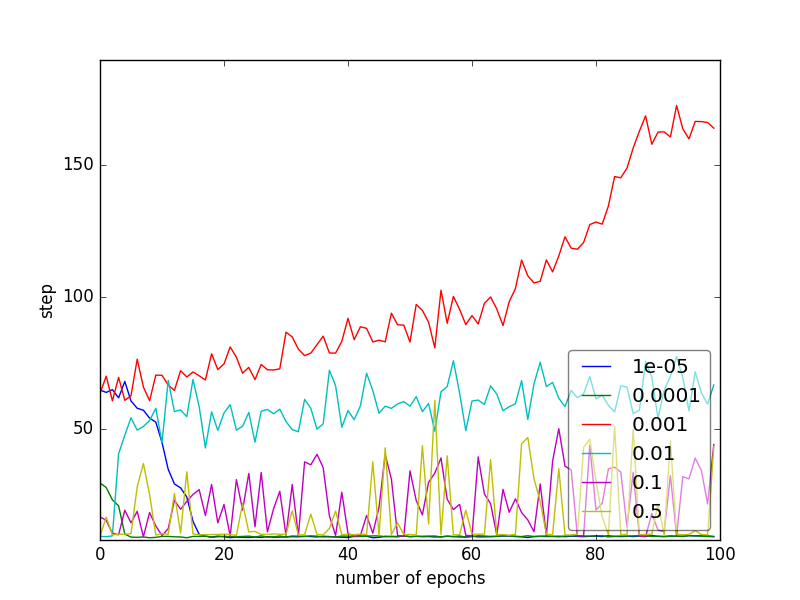
\includegraphics[width = \linewidth]{plots/a3-1/step.png}
\caption{test performance - average number of steps over 100 episodes }
\end{figure}

As it can be seen on the plot above, the model seems to learn best for learning rates of \textbf{0.001} or \textbf{0.01}. However, over 100 epochs, the systems doesn't converge yet which suggests it would require a longer training time.

\begin{figure}[H]
    \begin{minipage}[c]{.49\linewidth}
        \centering
        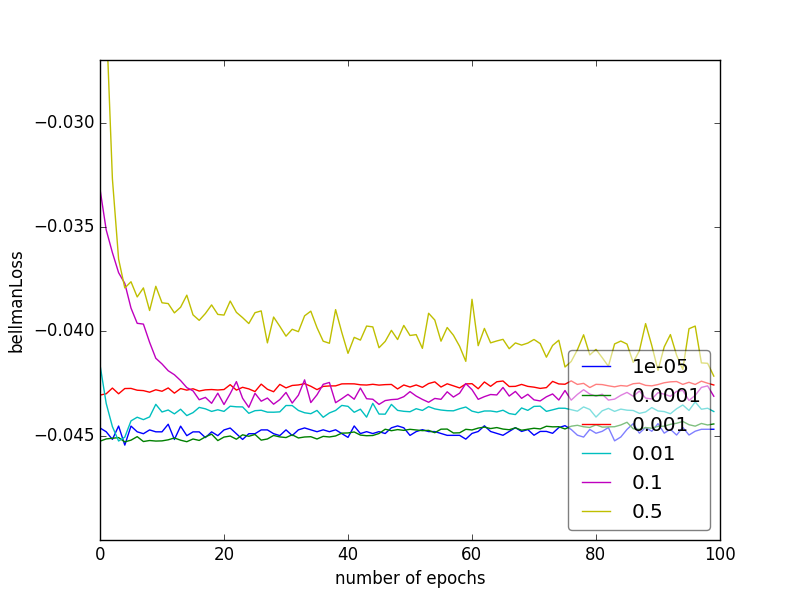
\includegraphics[width = 0.7\linewidth]{plots/a3-1/bellmanLoss.png}
        \caption{bellman residual}
    \end{minipage}
    \hfill%
    \begin{minipage}[c]{.49\linewidth}
        \centering
        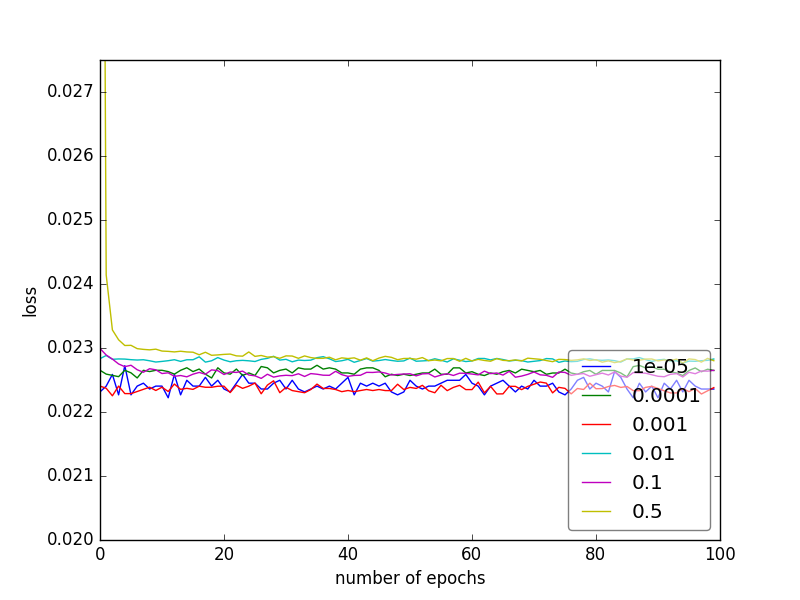
\includegraphics[width = 0.7\linewidth]{plots/a3-1/loss.png}
        \caption{Training Loss}
    \end{minipage}
\end{figure}

\subsubsection*{Part 2 : One hidden Layer}


\begin{figure}[H]
\centering
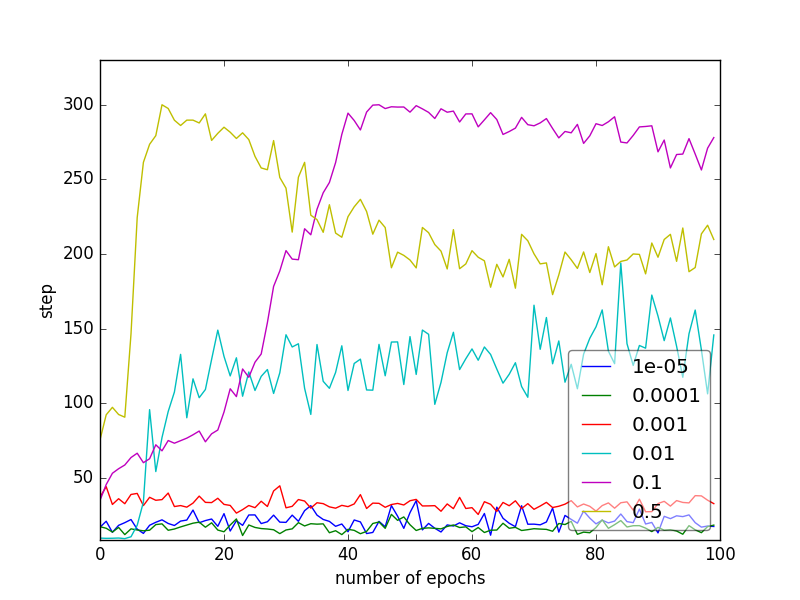
\includegraphics[width = \linewidth]{plots/a3-2/step.png}
\caption{test performance - average number of steps over 100 episodes }
\end{figure}


The second model seems to behave far better as it reaches the \textbf{300 steps} threshold set up for some of the attempted learning rates. In this case, the higher learning rates \textbf{(0.5,0.1,0.01)}. However, it seems that it quickly over fits for a learning rate of \textbf{0.5} and doesn't learn fast enough \textbf{0.01}. A learning rate of \textbf{0.1} then seems to be the optimal value.

\begin{figure}[H]
    \begin{minipage}[c]{.46\linewidth}
        \centering
        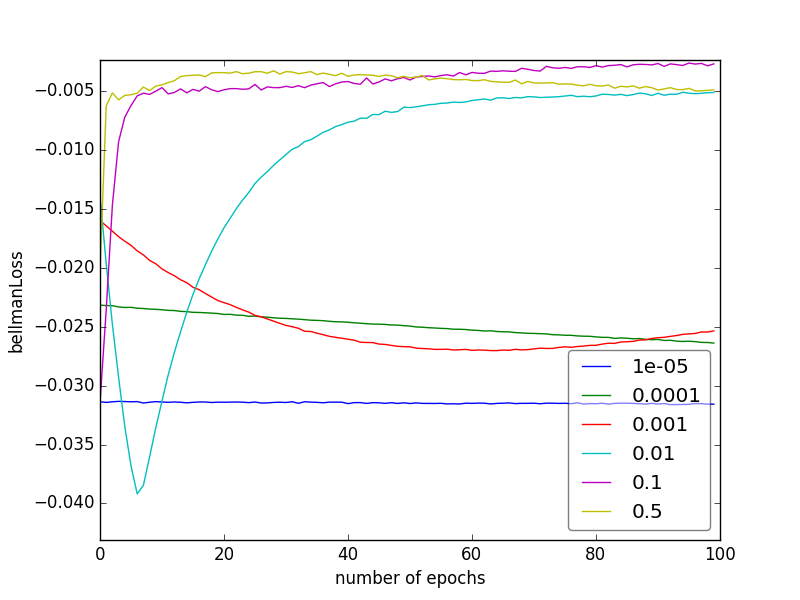
\includegraphics[width = 0.7\linewidth]{plots/a3-2/bellmanLoss.png}
        \caption{bellman residual}
    \end{minipage}
    \hfill%
    \begin{minipage}[c]{.46\linewidth}
        \centering
        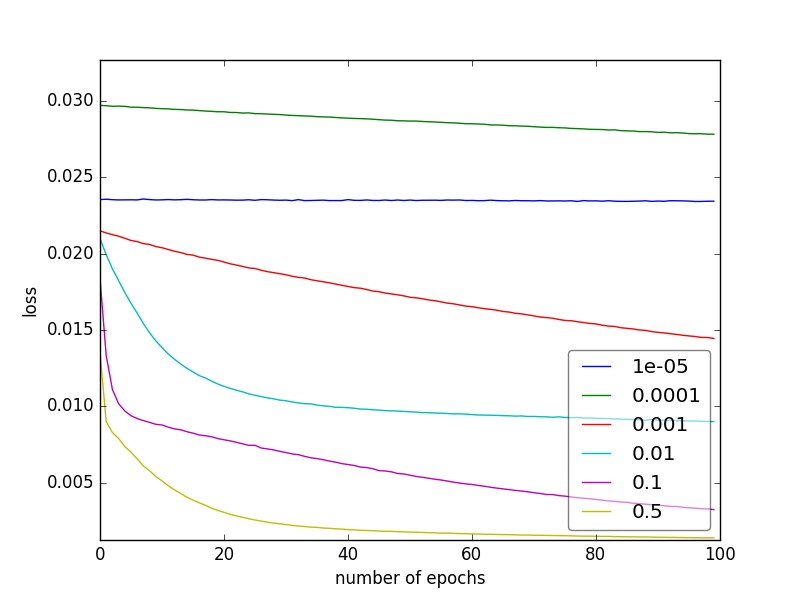
\includegraphics[width = 0.7\linewidth]{plots/a3-2/loss.png}
        \caption{Training Loss}
    \end{minipage}
\end{figure}

\subsection*{Question 4}

\begin{figure}[H]
\begin{minipage}[c]{.49\linewidth}
	\centering
	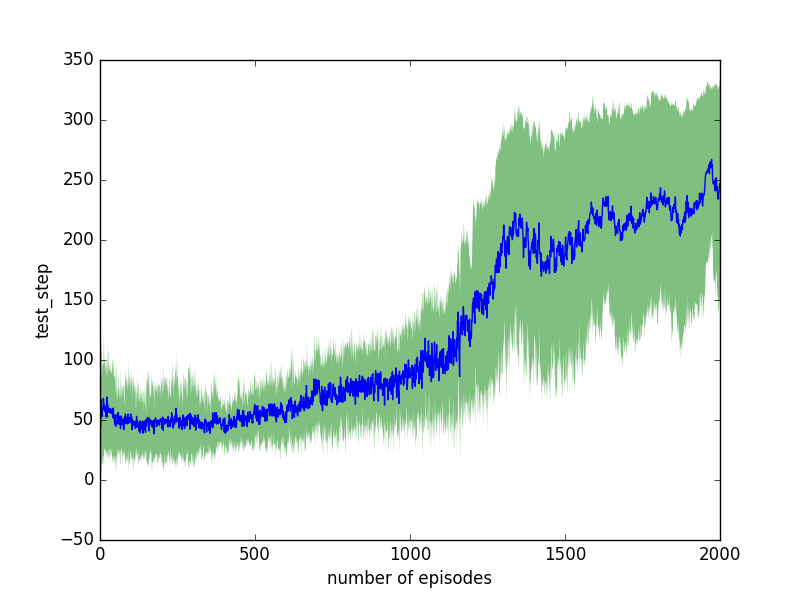
\includegraphics[width = \linewidth]{plots/a4/test_step.png}
	\caption{test performance}
    \end{minipage}
    \hfill%
\begin{minipage}[c]{.49\linewidth}
    \centering 
    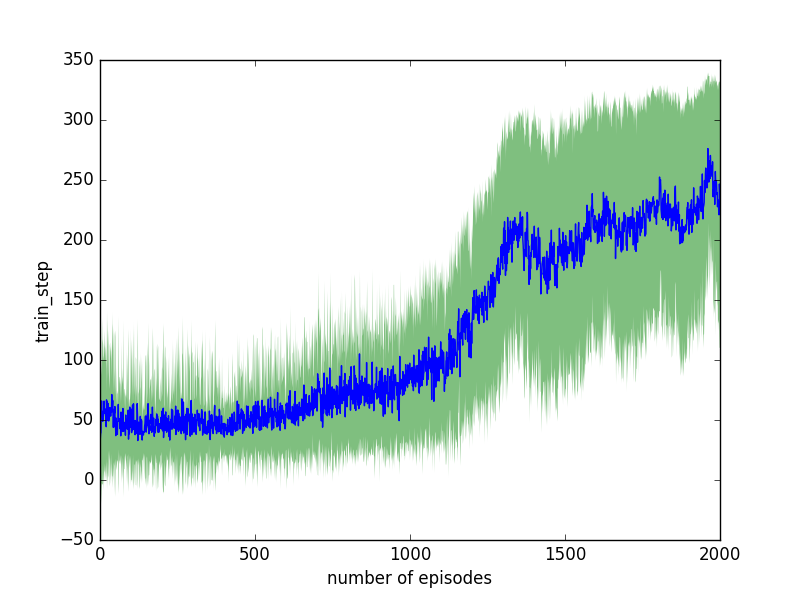
\includegraphics[width = \linewidth]{plots/a4/train_step.png}
	\caption{train performance}
\end{minipage}

\end{figure}
\begin{figure}[H]
    \begin{minipage}[c]{.49\linewidth}
        \centering
        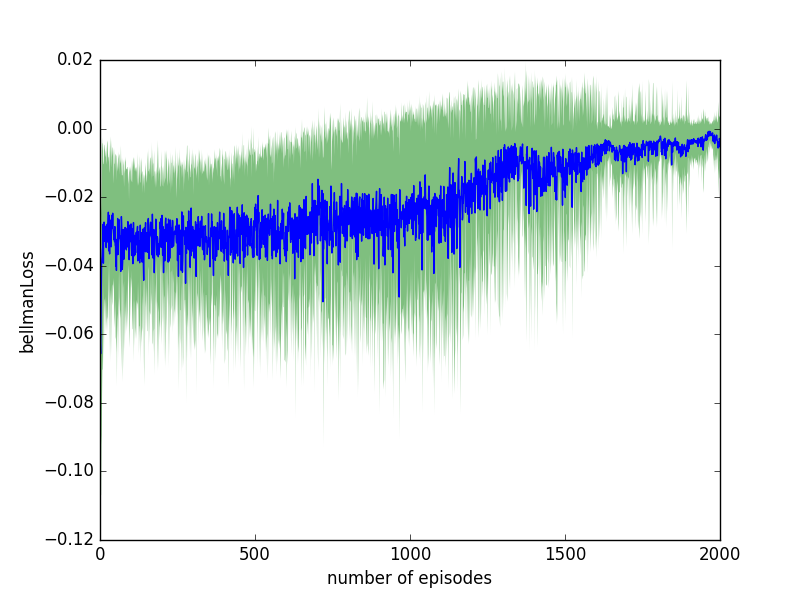
\includegraphics[width = \linewidth]{plots/a4/bellmanLoss.png}
        \caption{bellman residual}
    \end{minipage}
    \hfill%
    \begin{minipage}[c]{.49\linewidth}
        \centering
        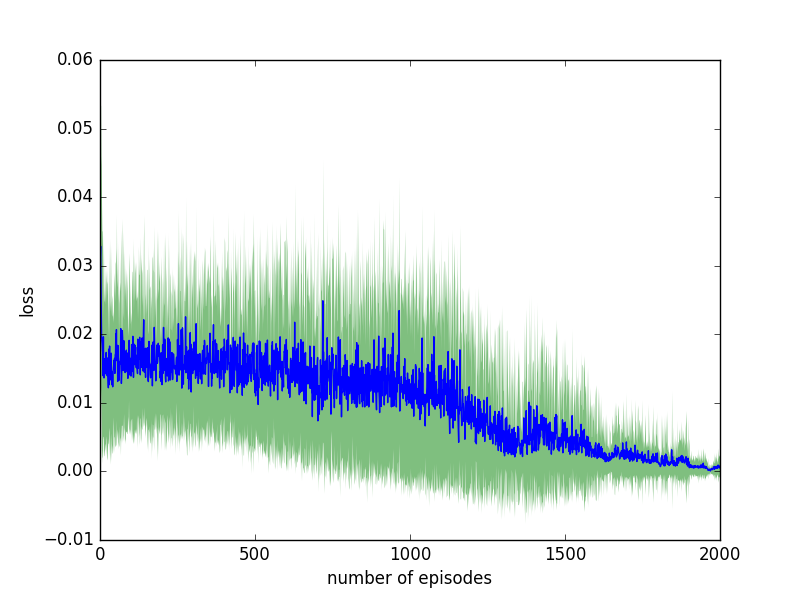
\includegraphics[width = \linewidth]{plots/a4/loss.png}
        \caption{Training Loss}
    \end{minipage}
\end{figure}


the plots displayed above are the results a Q-learning agent following an \textbf{$\epsilon$-greedy} policy during training with \textbf{$\epsilon = 0.05$} trained at every transition over 2000 episodes The learning Rate was chosen emperically to be \textbf{0.01} . This process was iterated 100 times and averaged, these plots display both the mean and the standard deviation of the following metrics : \textbf{[bellman residual, training loss, train episode lenght, test episodes length averaged over 10 episodes]}. As it can be noticed, the model does seem to learn properly as the average number of steps increases and the losses decreases, however, this process seems to be quite noise as the \textbf{standard deviation} remains high. 

\subsection*{Question 5}


\begin{figure}[H]
\begin{minipage}[c]{.49\linewidth}
	\centering
	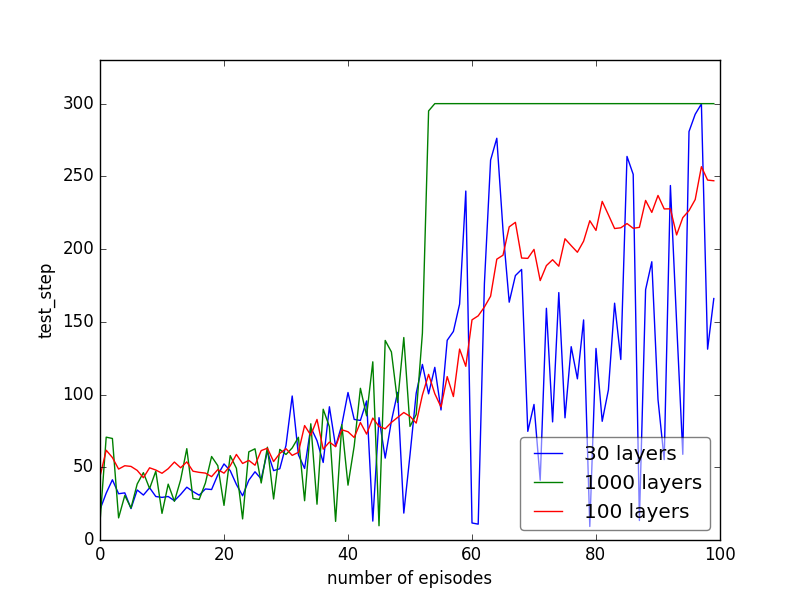
\includegraphics[width = \linewidth]{plots/a5/test_step.png}
	\caption{test performance}
    \end{minipage}
    \hfill%
\begin{minipage}[c]{.49\linewidth}
    \centering 
    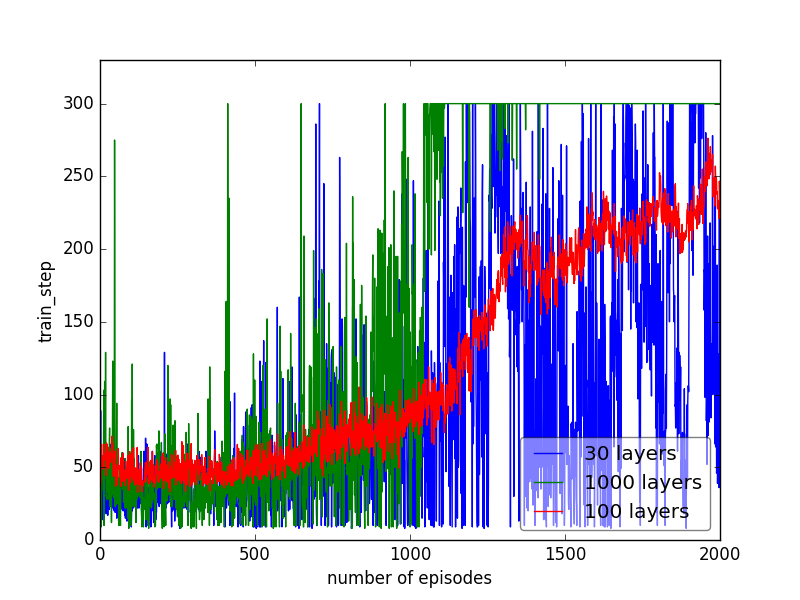
\includegraphics[width = \linewidth]{plots/a5/train_step.png}
	\caption{train performance}
\end{minipage}

\end{figure}
\begin{figure}[H]
    \begin{minipage}[c]{.49\linewidth}
        \centering
        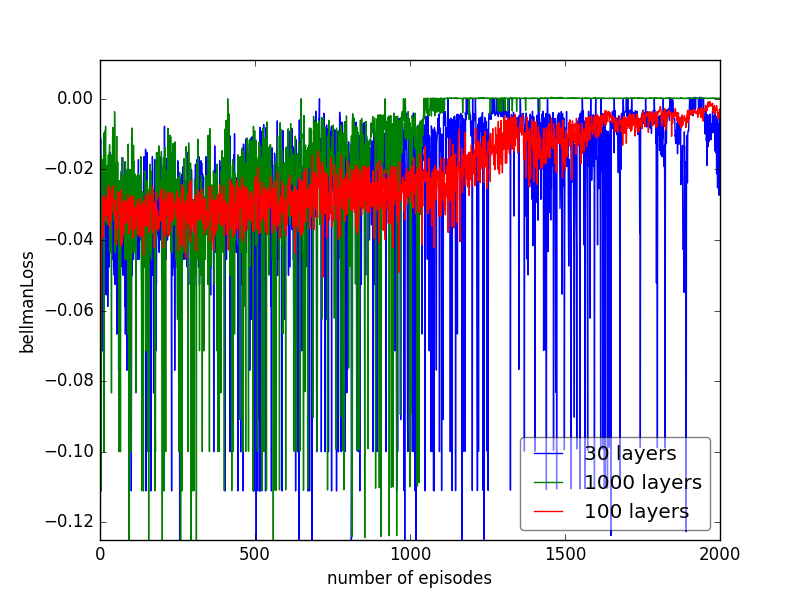
\includegraphics[width = \linewidth]{plots/a5/bellmanLoss.png}
        \caption{bellman residual}
    \end{minipage}
    \hfill%
    \begin{minipage}[c]{.49\linewidth}
        \centering
        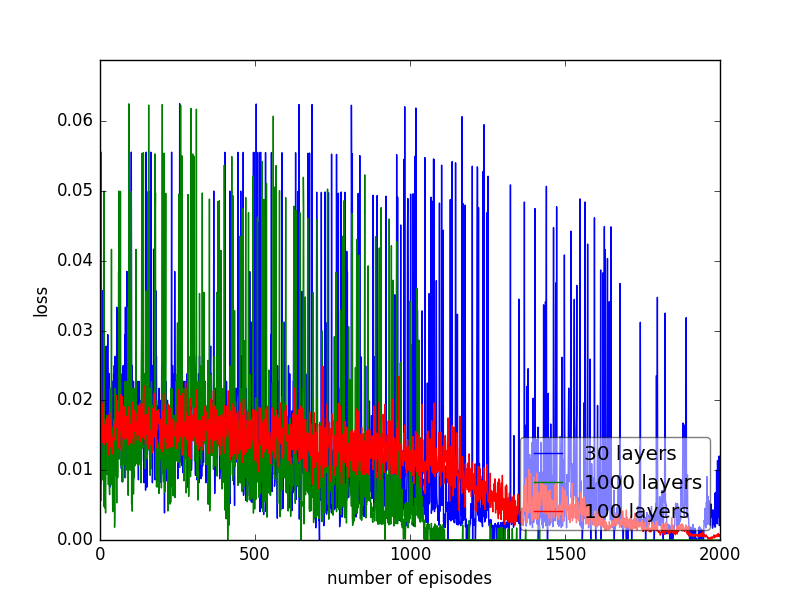
\includegraphics[width = \linewidth]{plots/a5/loss.png}
        \caption{Training Loss}
    \end{minipage}
\end{figure}


We then tried to assess the importance of the hidden layer size, by comparing the previous results to a the same network with first a \textbf{hidden layer size of 30} and then a \textbf{hidden layer size of 1000}. In order to be able to fairly compare the models, we keep the learning rate fixed to  \textbf{0.01}. As expected, increasing the hidden size seems to improve the learning process, as the model with 30 neurones displays worse performance than the initial one and the 1000 neurones model converges faster \textit{within 1200 episodes} and remains reliably at the maximal performance possible . 

\subsection*{Question 6}

\begin{figure}[H]
\begin{minipage}[c]{.49\linewidth}
	\centering
	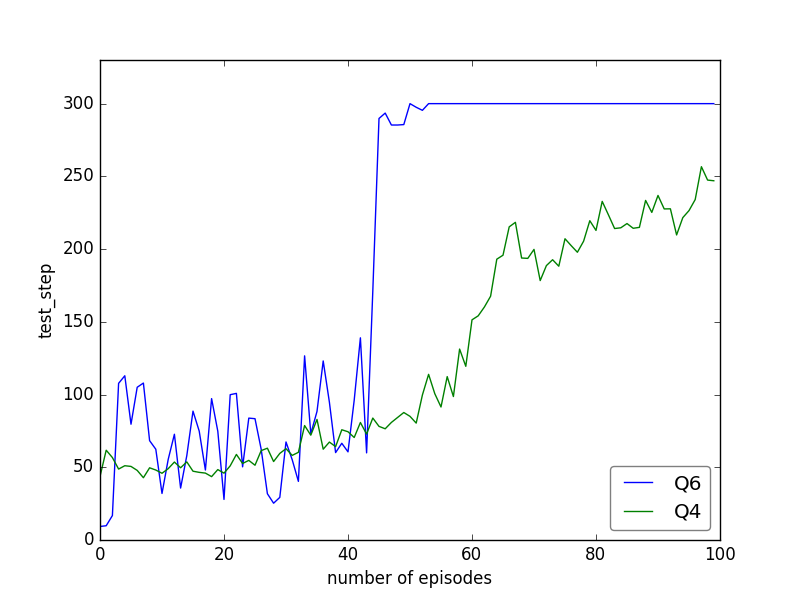
\includegraphics[width = \linewidth]{plots/a6/test_step.png}
	\caption{test performance}
    \end{minipage}
    \hfill%
\begin{minipage}[c]{.49\linewidth}
    \centering 
    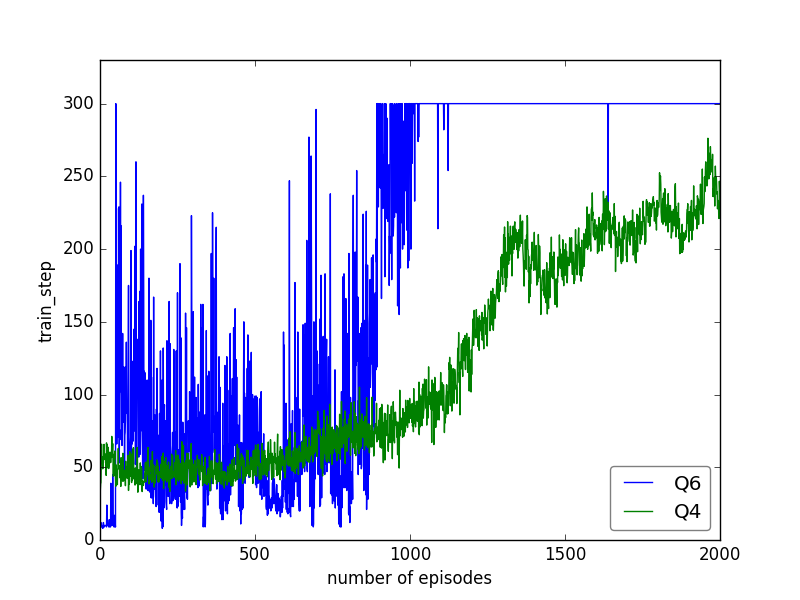
\includegraphics[width = \linewidth]{plots/a6/train_step.png}
	\caption{train performance}
\end{minipage}

\end{figure}
\begin{figure}[H]
    \begin{minipage}[c]{.49\linewidth}
        \centering
        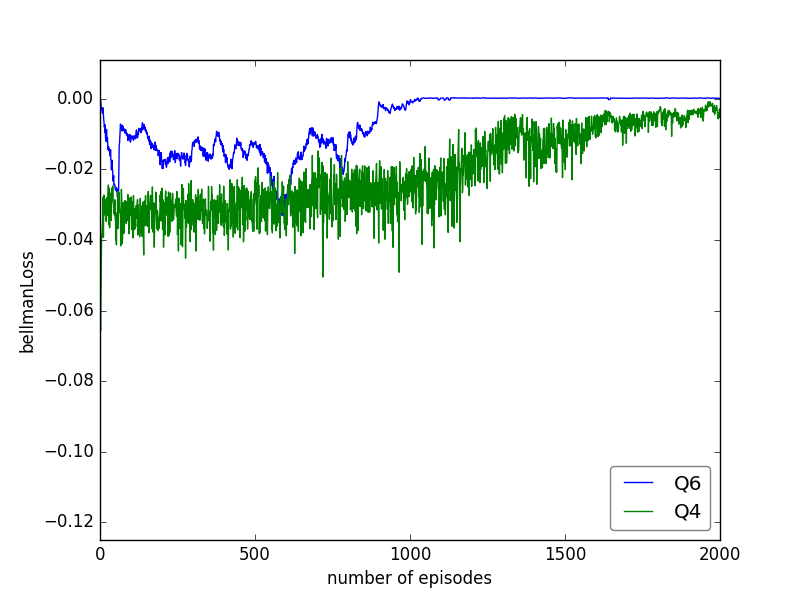
\includegraphics[width = \linewidth]{plots/a6/bellmanLoss.png}
        \caption{bellman residual}
    \end{minipage}
    \hfill%
    \begin{minipage}[c]{.49\linewidth}
        \centering
        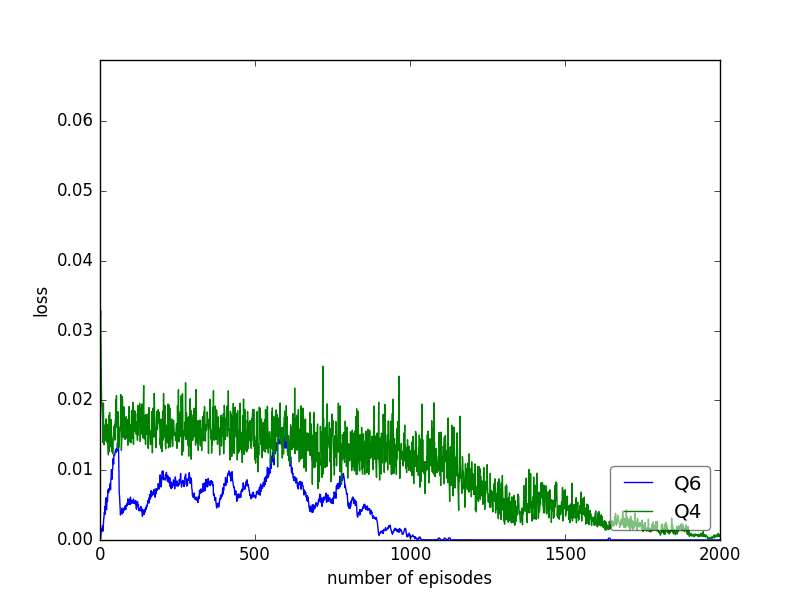
\includegraphics[width = \linewidth]{plots/a6/loss.png}
        \caption{Training Loss}
    \end{minipage}
\end{figure}

We then implemented a replay buffer, in order to try to improve the results obtained above. After a few attempts, The \textbf{buffer size was set to 2000} and the \textbf{batch size to 500} and the \textbf{learning rate to 0.015}. As it can be seen above, this model was more performant than any of the three models attempted in question 4 and 5. It converged within 1000 episodes and remained consistent. As the loss can prove it, this model also seems to be less noisy than the one implemented before.

\subsection*{Question 7}

\begin{figure}[H]
\begin{minipage}[c]{.49\linewidth}
	\centering
	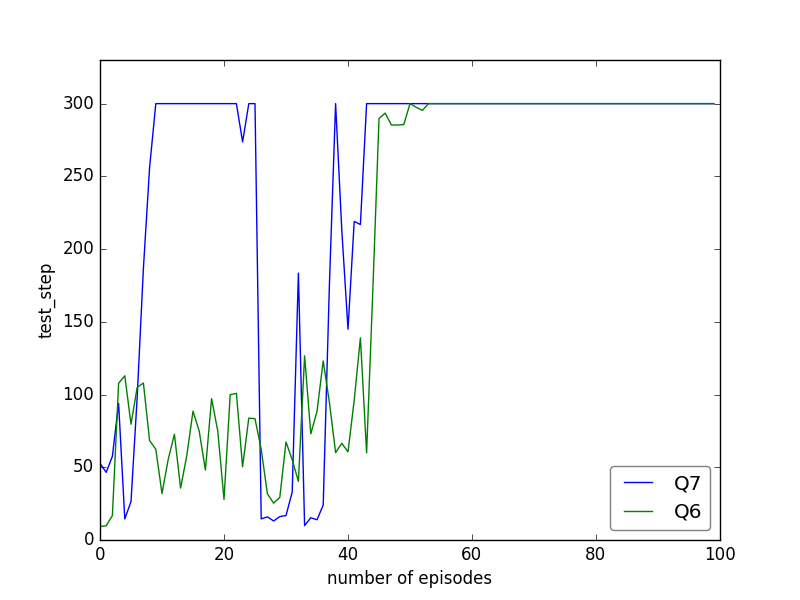
\includegraphics[width = \linewidth]{plots/a7/test_step.png}
	\caption{test performance}
    \end{minipage}
    \hfill%
\begin{minipage}[c]{.49\linewidth}
    \centering 
    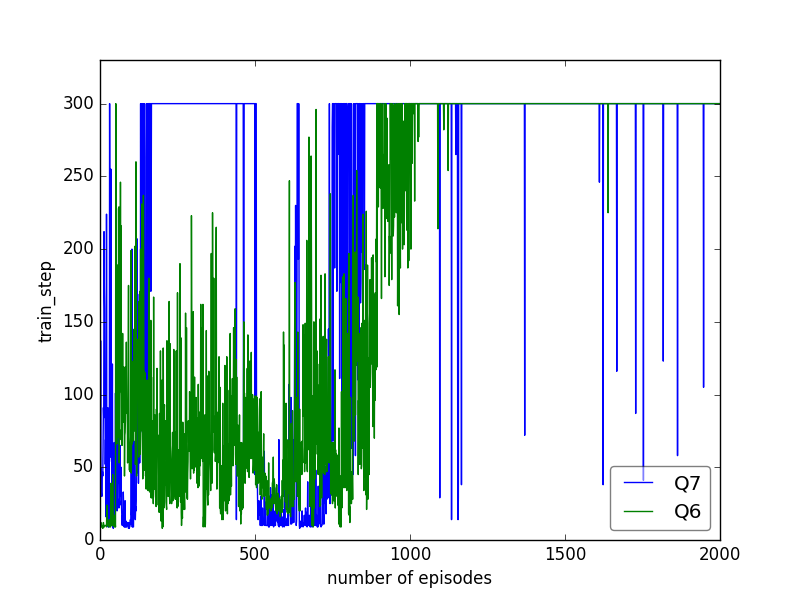
\includegraphics[width = \linewidth]{plots/a7/train_step.png}
	\caption{train performance}
\end{minipage}

\end{figure}
\begin{figure}[H]
    \begin{minipage}[c]{.49\linewidth}
        \centering
        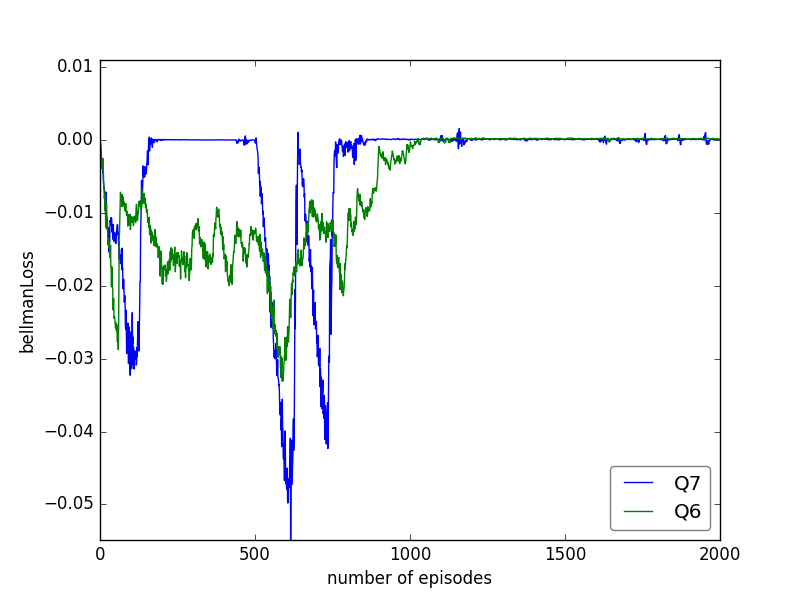
\includegraphics[width = \linewidth]{plots/a7/bellmanLoss.png}
        \caption{bellman residual}
    \end{minipage}
    \hfill%
    \begin{minipage}[c]{.49\linewidth}
        \centering
        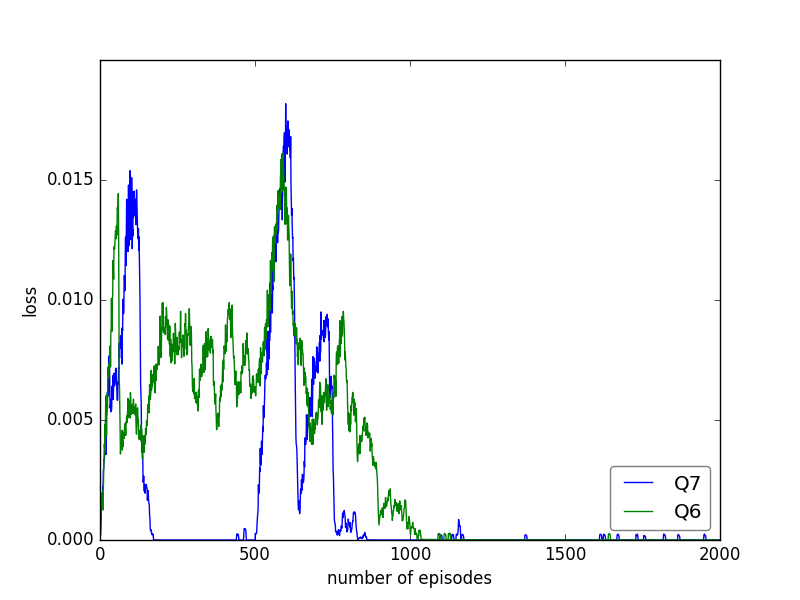
\includegraphics[width = \linewidth]{plots/a7/loss.png}
        \caption{Training Loss}
    \end{minipage}
\end{figure}

In order to continue improving the model, we modified the neural network implementation to add a target network that was updated every \textbf{5 episodes} (this was done by using the \textit{tensorflow assign operation}) and combined with the buffer replay implemented before. This model was trained using the parameters presented in question 6, the sole difference being the \textbf{the learning rate that was set to 0.00001}. The results for this model were plotted against the previous model \textit{(question 6)} in order to be able to clearly see the improvements. Indeed, this model seems to be even better than what was implemented above as it \textbf{converges in less than 800 episodes}. 


\subsection*{Question 8}

\begin{figure}[H]
\begin{minipage}[c]{.49\linewidth}
	\centering
	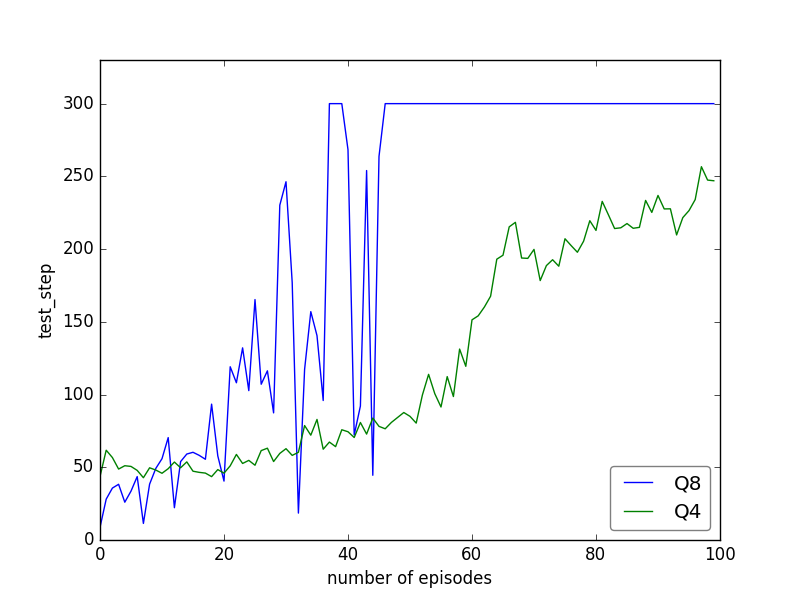
\includegraphics[width = \linewidth]{plots/a8/test_step.png}
	\caption{test performance}
    \end{minipage}
    \hfill%
\begin{minipage}[c]{.49\linewidth}
    \centering 
    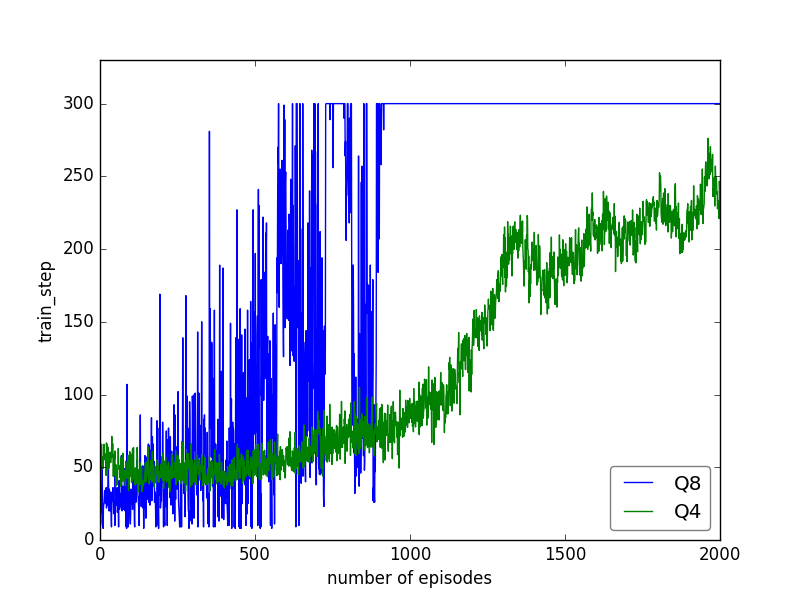
\includegraphics[width = \linewidth]{plots/a8/train_step.png}
	\caption{train performance}
\end{minipage}

\end{figure}
\begin{figure}[H]
    \begin{minipage}[c]{.49\linewidth}
        \centering
        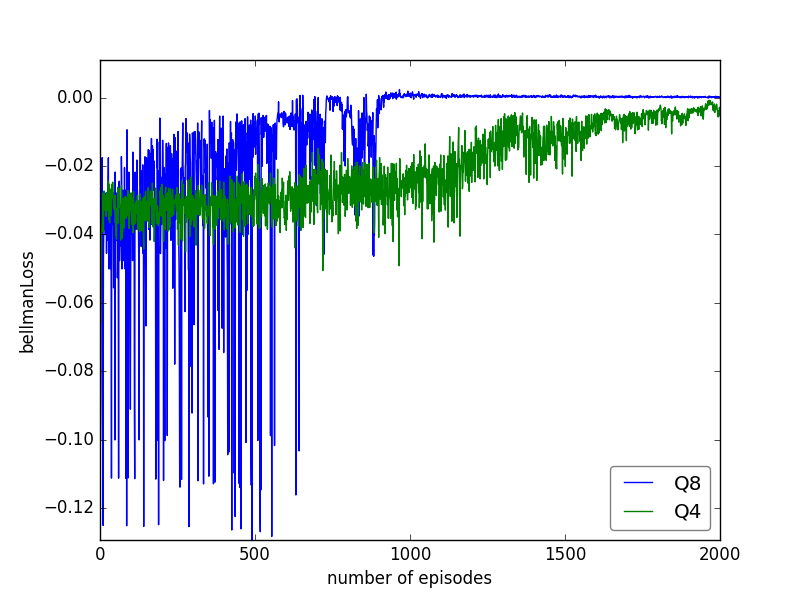
\includegraphics[width = \linewidth]{plots/a8/bellmanLoss.png}
        \caption{bellman residual}
    \end{minipage}
    \hfill%
    \begin{minipage}[c]{.49\linewidth}
        \centering
        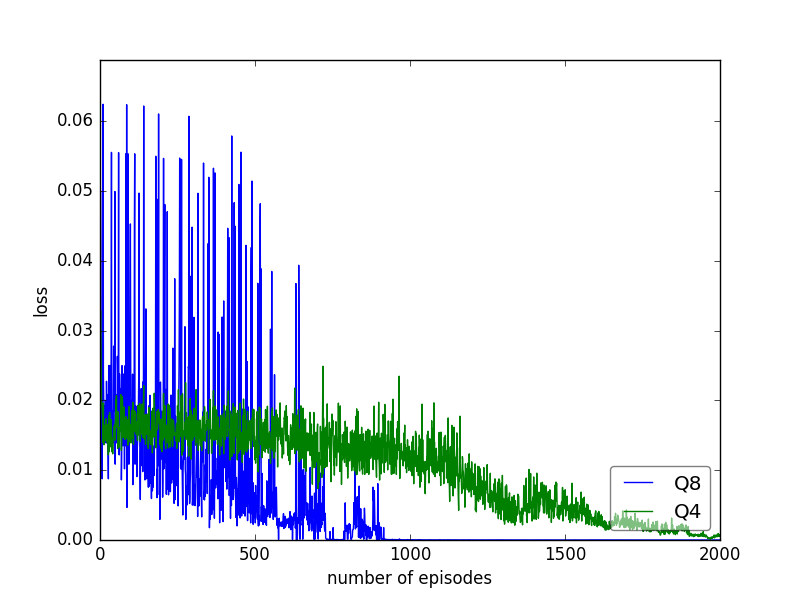
\includegraphics[width = \linewidth]{plots/a8/loss.png}
        \caption{Training Loss}
    \end{minipage}
\end{figure}


Finally, we implemented a Double-Q learning Agent in order to compare its performance with a simple Q-learning agent. In order to be able to properly compare this model with the model implemented in question 4, it was not combined with a replay buffer. The learning rate chosen for this model was \textbf{0.035}. The performance reached by this algorithm is comparable to the ones reached by the model combining a target network and a replay buffer. It converges to the maximum threshold in \textbf{less than 1000 episodes}.

\newpage

\section*{II - Problem B}

\subsection*{Question 1}

bellow are the mean and standard deviation for both the cumulative discounted score as well as the frame count under a \textbf{random policy} for each game  over 100 episodes .  \\

\begin{table}[H]
\centering
\label{b1Tab}
\begin{tabular}{c|c|c|c|c|c|c|}
\cline{2-7}
& \multicolumn{2}{c|}{Ms Pacman} & \multicolumn{2}{c|}{Pong} & \multicolumn{2}{c|}{Boxer} \\ 
\cline{2-7}  & Score       & Frame count      & Score    & Frame count & Score  & Frame count    \\ \hline
\multicolumn{1}{|c|}{mean}     &  2.56 & 670.3   &  -0.84  & 1019.43  & -0.24   &  2378.14  \\ \hline
\multicolumn{1}{|c|}{standard deviation} &  0.74  &  105.5 &     0.36      &    9.377   &       1.13    & 12.73  \\ \hline
\end{tabular}
\caption{mean and standard deviation for score and frame count averaged over 100 episodes for all games obtained following a random policy}
\end{table}

\subsection*{Question 2}


bellow are the mean and standard deviation for both the cumulative discounted score as well as the frame count under a \textbf{greedy policy using an untrained model} for each game  over 100 episodes .  \\
\begin{table}[H]
\centering
\caption{mean and standard deviation for score and frame count averaged over 100 episodes for all games obtained following an untrained neural network}
\label{b2Tab}
\begin{tabular}{c|c|c|c|c|c|c|}
\cline{2-7}
& \multicolumn{2}{c|}{Ms Pacman} & \multicolumn{2}{c|}{Pong} & \multicolumn{2}{c|}{Boxer} \\ 
\cline{2-7}  & Score       & Frame count      & Score    & Frame count & Score  & Frame count    \\ \hline
\multicolumn{1}{|c|}{mean}     &  2.50 & 627.73   &  -1.14  & 1019.36  &  -0.38  &  2379.62  \\ \hline
\multicolumn{1}{|c|}{standard deviation} &  0.07  &  6.34  &     0.03      &    9.68   &        0.075    & 13.55  \\ \hline
\end{tabular}
\end{table}

Two main differences exists between the results obtained here and the results obtained above:
\begin{itemize}
	\item \textbf{the standard deviation}  is consistently smaller in the second case
	\item \textbf{the score}: is consistently worse for the untrained model than for a random policy
\end{itemize}

This is due to the fact that while \textbf{a random policy will always randomly pick an action to take}, an \textbf{untrained model will nearly always take the same action} as it is a deterministic process. Indeed, when the convultion layers are not trained, the untrained model is metaphorically \textit{blind} as it cannot identify any interesting feature, it is then quite likely always take the same action which would mean obtaining the same (likely bad) outcome everytime hence the smaller standard deviation and cumulative score.

\subsection*{Question 3}

After initially training the model under the parameters specified in the assignment, we tried lowering the learning rate to 0.0001 as the system was not performing well for the initial parameters. Furthermore, in order to improve the performance, we also tried increasing the preprocessed image size to \textbf{60x60}. Bellow are presented the results for all attempts made.  

\subsubsection*{Boxing}

\begin{figure}[H]
    \begin{minipage}[c]{.49\linewidth}
        \centering
        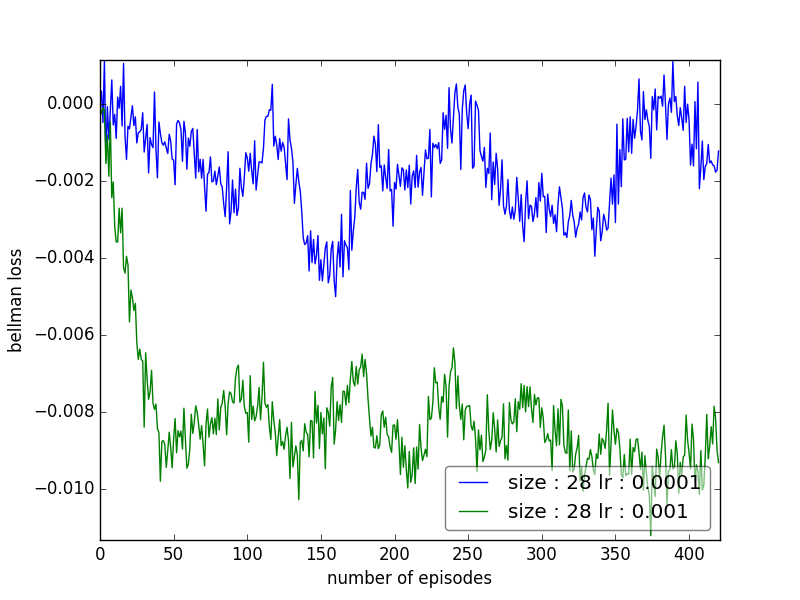
\includegraphics[width = \linewidth]{plots/b3/Boxing-v3/bellmanLossArray.png}
        \caption{bellman residual}
    \end{minipage}
    \hfill%
    \begin{minipage}[c]{.49\linewidth}
        \centering
        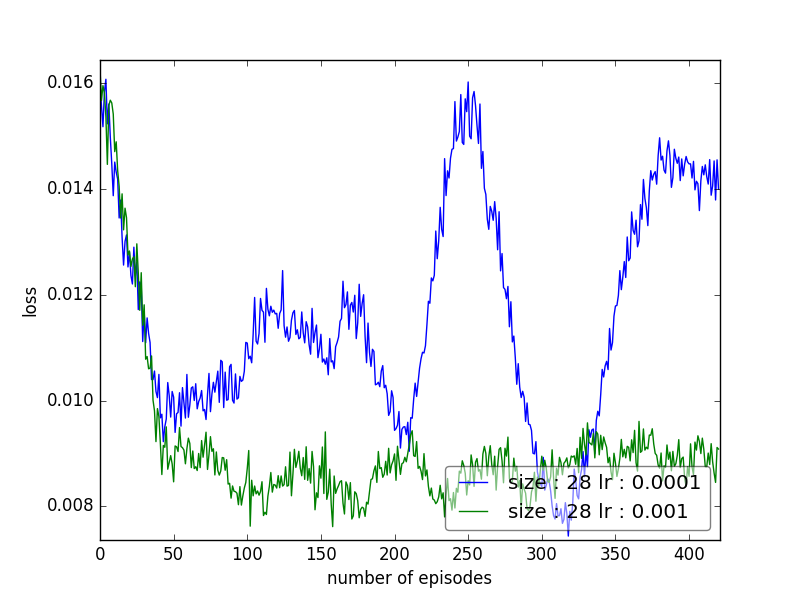
\includegraphics[width = \linewidth]{plots/b3/Boxing-v3/lossArray.png}
        \caption{Training Loss}
    \end{minipage}
\end{figure}

\subsubsection*{Ms Pacman}


\begin{figure}[H]
    \begin{minipage}[c]{.49\linewidth}
        \centering
        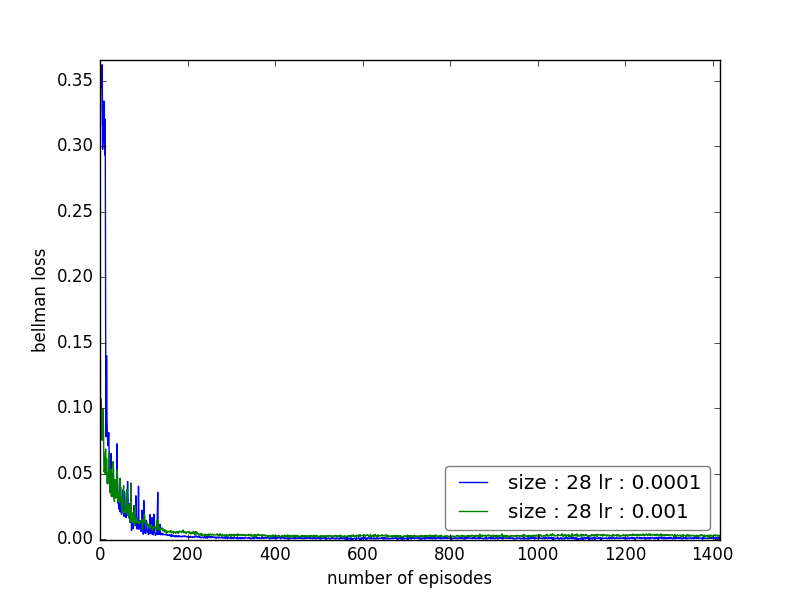
\includegraphics[width = \linewidth]{plots/b3/MsPacman-v3/bellmanLossArray.png}
        \caption{bellman residual}
    \end{minipage}
    \hfill%
    \begin{minipage}[c]{.49\linewidth}
        \centering
        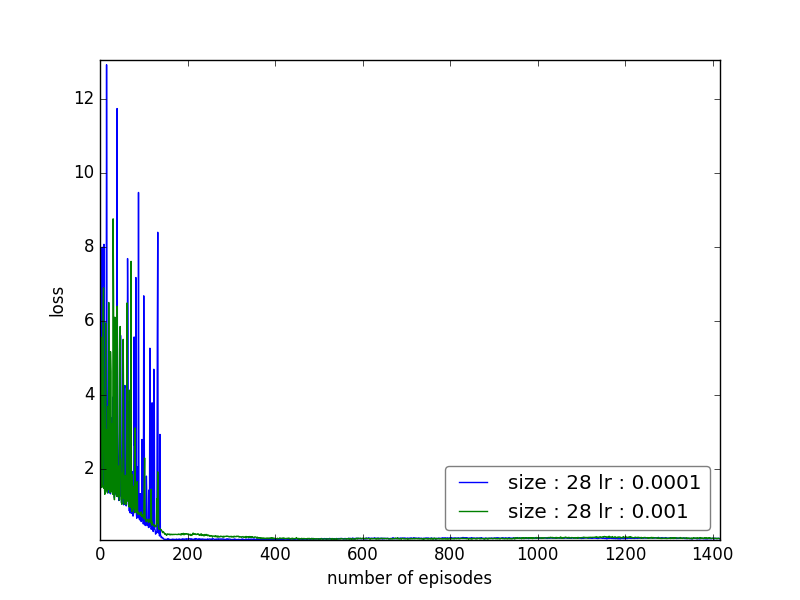
\includegraphics[width = \linewidth]{plots/b3/MsPacman-v3/lossArray.png}
        \caption{Training Loss}
    \end{minipage}
\end{figure}

\subsubsection*{Pong}


\begin{figure}[H]
    \begin{minipage}[c]{.49\linewidth}
        \centering
        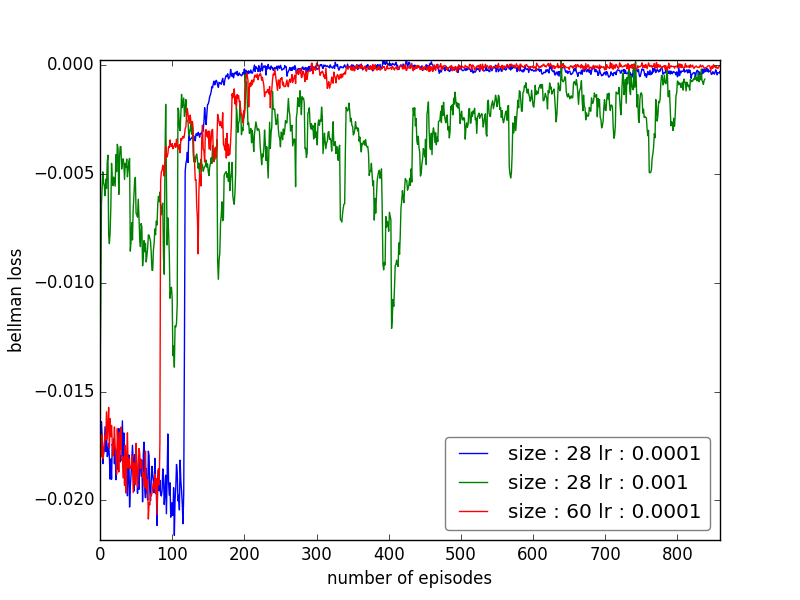
\includegraphics[width = \linewidth]{plots/b3/Pong-v3/bellmanLossArray.png}
        \caption{bellman residual}
    \end{minipage}
    \hfill%
    \begin{minipage}[c]{.49\linewidth}
        \centering
        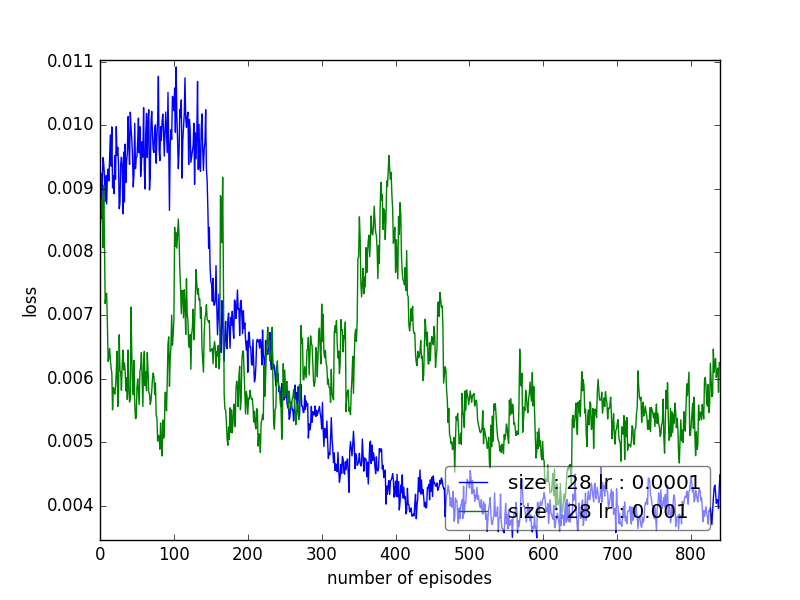
\includegraphics[width = \linewidth]{plots/b3/Pong-v3/lossArray.png}
        \caption{Training Loss}
    \end{minipage}
\end{figure}


Overall, it seems that the \textbf{loss decreases} and \textbf{the bellman loss} gets closer to zero for a smaller learning rate of 0.0001 with the exception of \textbf{boxer} game where the loss decreases for a higher learning rate of 0.001. However, these plots differ from a supervised learning case because, as opposed to the supervised learning where the loss would correlated with whether or not the agent took the right action, in this case the loss can decrease even though the system is not learning the targeted behaviour. as it aims to accurately predict its cumulative reward and not maximize it.


\subsection*{Question 4}


\subsubsection*{Boxing}


\begin{figure}[H]
\begin{minipage}[c]{.49\linewidth}
	\centering
	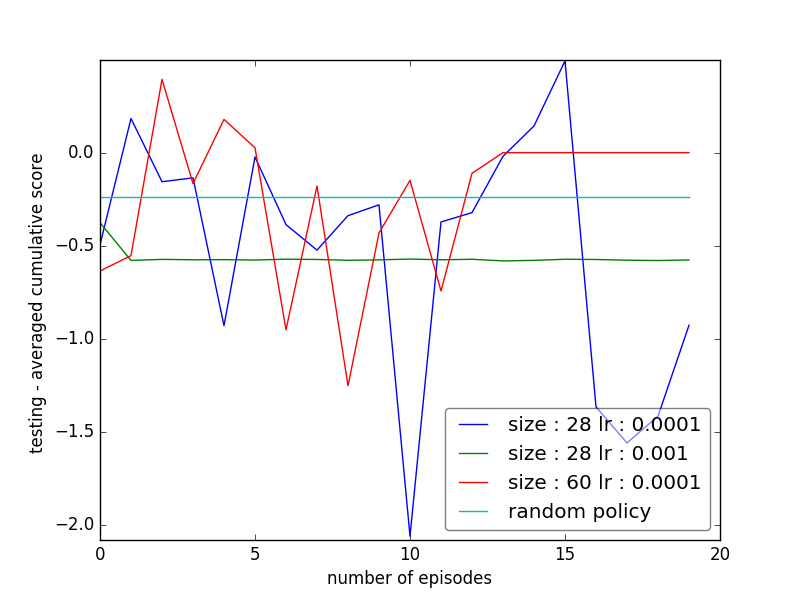
\includegraphics[width = \linewidth]{plots/b3/Boxing-v3/testScoreMean.png}
	\caption{test performance}
    \end{minipage}
    \hfill%
\begin{minipage}[c]{.49\linewidth}
    \centering 
    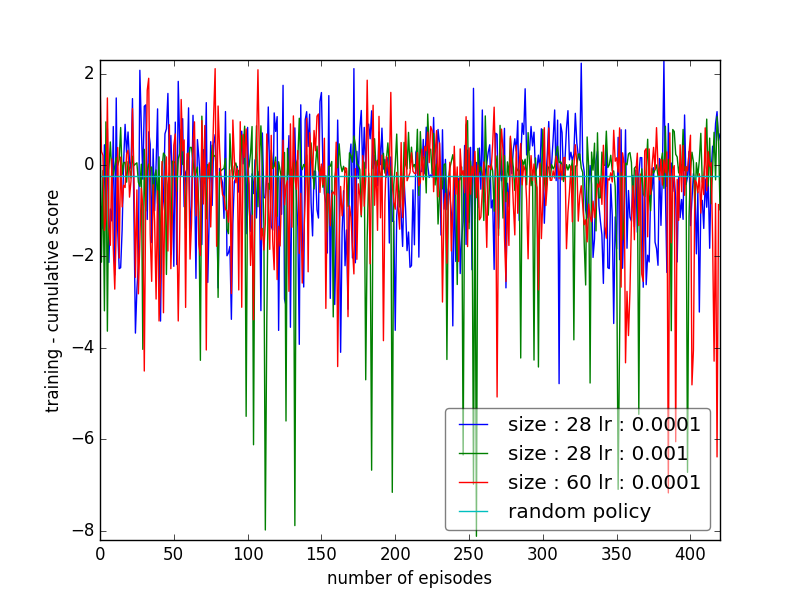
\includegraphics[width = \linewidth]{plots/b3/Boxing-v3/trainScore.png}
	\caption{train performance}
\end{minipage}
\end{figure}

\subsubsection*{Ms Pacman}


\begin{figure}[H]
\begin{minipage}[c]{.49\linewidth}
	\centering
	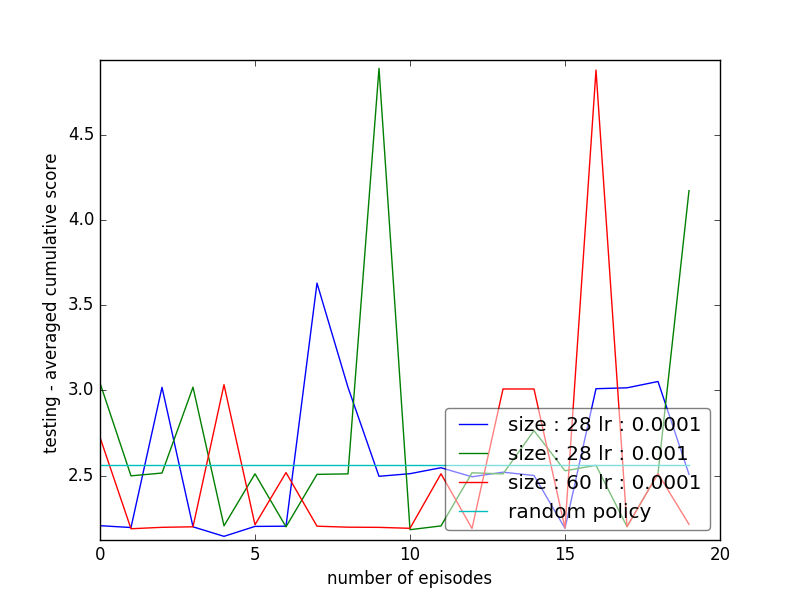
\includegraphics[width = \linewidth]{plots/b3/MsPacman-v3/testScoreMean.png}
	\caption{test performance}
    \end{minipage}
    \hfill%
\begin{minipage}[c]{.49\linewidth}
    \centering 
    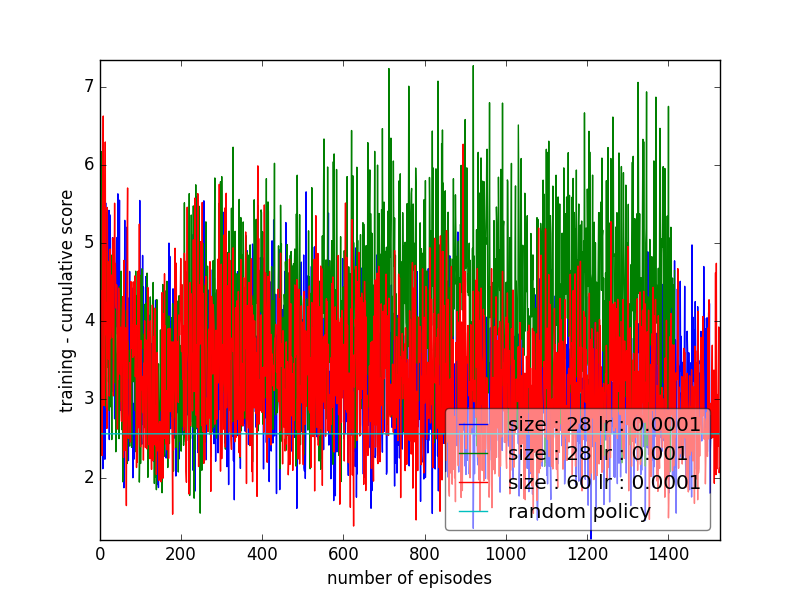
\includegraphics[width = \linewidth]{plots/b3/MsPacman-v3/trainScore.png}
	\caption{train performance}
\end{minipage}
\end{figure}

\subsubsection*{Pong}

\begin{figure}[H]
\begin{minipage}[c]{.49\linewidth}
	\centering
	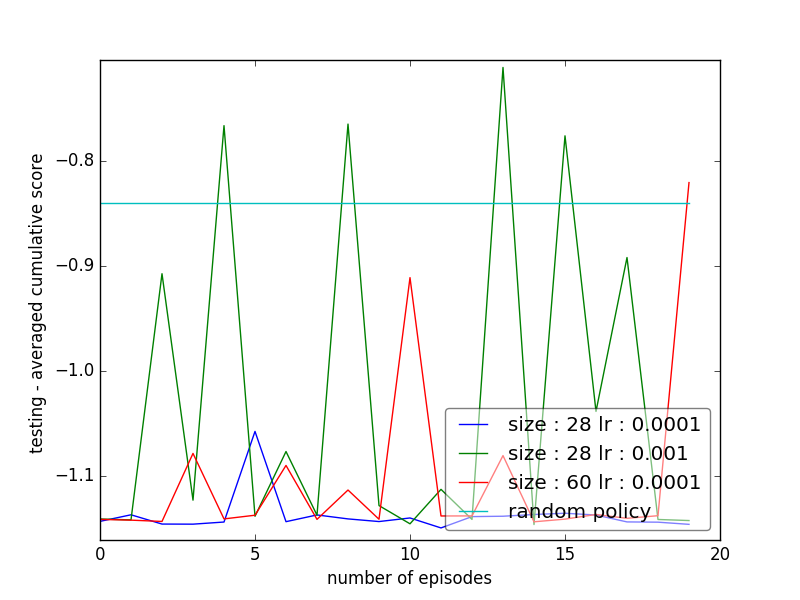
\includegraphics[width = \linewidth]{plots/b3/Pong-v3/testScoreMean.png}
	\caption{test performance}
    \end{minipage}
    \hfill%
\begin{minipage}[c]{.49\linewidth}
    \centering 
    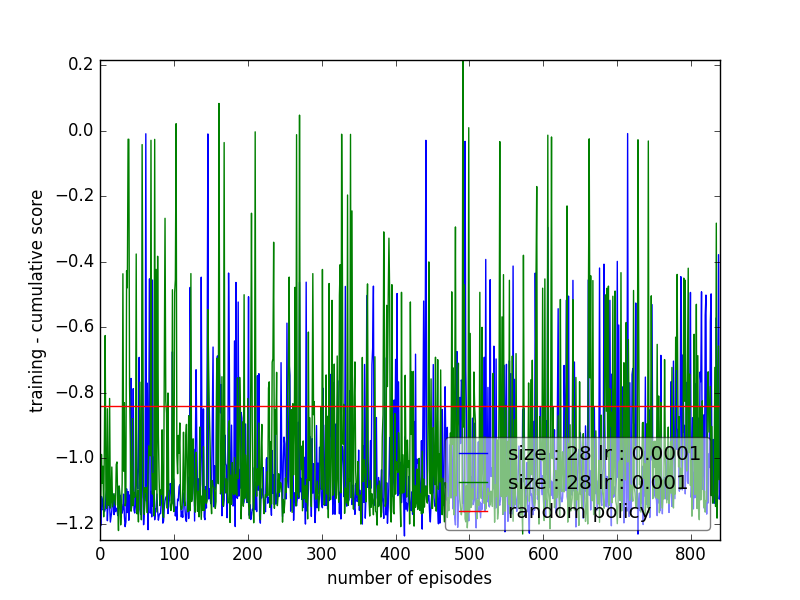
\includegraphics[width = \linewidth]{plots/b3/Pong-v3/trainScore.png}
	\caption{train performance}
\end{minipage}
\end{figure}


here are the final cumulative discounted scores (tested on the best model saved) obtained for each attempt: \\

\begin{table}[H]
\centering
\label{b4Tab}
\begin{tabular}{|c|c|c|c|}
\hline
settings 				& Ms Pacman 		& Pong 				& Boxer 		  \\ \hline
size : 28, lr : 0.0001  & 3.61 				& -1.08 			& \textbf{0.66}   \\ \hline
size : 28, lr : 0.001  	& 4.87 				& \textbf{-0.81} 	& -0.37 		  \\ \hline
size : 60, lr : 0.0001  & \textbf{4.944} 	& -1.14 			& 0.51	 		  \\ \hline
\textit{random policy} 	& \textit{2.56} 	& \textit{-0.84}	& \textit{-0.24}  \\ \hline
\end{tabular}


\caption{final cumulative scores averaged over 100 test epsiodes and compared with the results for a random policy }
\end{table}

Overall, it seems that increasing the preprocessed image size does seem to increase performance. As it can be seen above, the optimal settings  for each games are the following : 

\begin{itemize}
	\item \textbf{Ms PacMan} : size 60 and learning rate : 0.0001
	\item \textbf{Pong} : size 28 and learning rate : 0.001
	\item \textbf{Boxer} : size 28 and learning rate : 0.0001
\end{itemize}

Overall, it seems that \textbf{increasing the preprocessing image size} helps with the performance, as both MsPacman and Boxer have a performance that is better than a random policy for a size of 60. However, more parameter tuning is required in order to get a proper learning curve where the cumulative reward is consistently increase and converge to a high value. \textbf{cropping useless information from the images such as the score or the number of lives} as well as trying a bigger range of learning rates might be good methods to improve the results.

\end{document}